\documentclass[a4paper, oneside]{recipe}
\usepackage[ngerman]{babel}
\usepackage[utf8]{inputenc}
\usepackage[T1]{fontenc}
\usepackage{bookman}
\usepackage{nicefrac}
\usepackage{hyperref}
\usepackage{ccicons}
\usepackage{graphicx}
\usepackage{subfig}
\hypersetup{
    colorlinks=true,
    linkcolor=blue,
    filecolor=blue,      
    urlcolor=blue,
    pdftitle={Hefe-Zimt_zopf},
    pdfpagemode=FullScreen,
}
\newcommand{\bsi}[2]{%
  \fontencoding{T1}\fontfamily{pbs}\fontseries{xl}\fontshape{n}%
  \fontsize{#1}{#2}\selectfont}

\renewcommand{\inghead}{\textbf{Zutaten}:\ }
\renewcommand{\rechead}{\centering\bsi{24pt}{30pt}}
\makeatletter
\renewcommand*\l@subsubsection{\@dottedtocline{3}{3em}{0em}}
\makeatother
\setlength\parindent{0pt}
\setlength\parskip{2ex plus 0.5ex}
\begin{document}


\recipe{Hefe-Zimt-Zopf}
\ingred{250 ml Milch, 375 g Weizenmehl (Typ 405), 120 g Zucker, 1 Packung Trockenhefe (7 g), 150 g Butter (Zimmertemperatur), 1 Prise Salz, (1 Ei), 3 TL Zimt}

\section*{Vorwort}
Dies ist ein Rezept für ein Hefe-Zimt-Zopf, inspiriert von den Rezepten für einen Hefezopf\footnote{\url{https://www.einfachbacken.de/rezepte/hefezopf}} und für Zimtschnecken\footnote{\url{https://www.einfachbacken.de/rezepte/zimtschnecken-einfach-selbstgemacht}}. Umgesetzt von Fabian Belzner.\\

Stand: Februar 2023

\section*{Hefeteig}
\subsection*{Autolyse}
Mehl, Milch, 50 g Zucker, Hefe und 1 Prise Salz mit einem Kochlöffel in einer Schüssel so lange vermischen, bis das Mehl abbindet und keine trockenen Stellen mehr zu erkennen sind. Das Ganze 20 Minuten an einem warmen Ort stehen lassen. In dieser Zeit bildet sich die Glutenstrucktur des Teigs, was für die spätere Stabilität wichtig ist. Das braucht man spätestens beim Flechten.

\subsection*{Zubereitung}
Den Teig in eine Küchenmaschine geben und erst auf kleiner, dann auf höherer Stufe kneten und dabei das Ei und 50 g Butter stückchenweise zugeben. Der Teig ist dann fertig geknetet, wenn er sich vom Rand der Schüssel ablöst und nicht mehr klebrig ist. Jetzt sollte sich eine elastische Masse gebildet haben. Der ganze Knetvorgang dauert etwa 10 Minuten. Das Ei habe ich schon vergessen, was zu keinem schlechteren Ergebnis (eher besser!) geführt hat.

\subsection*{Stockgare}
Den Teig jetzt an einem warmen Ort für etwa 60 Minuten gehen lassen bis sich das Volumen deutlich vergrößert hat. Das ist ein biologischer Prozess, der u.a. von der Hefe und den Umgebungsbedingungen abhängig ist und somit länger oder kürzer gehen kann. Falls sich das Volumen nach 60 Minuten noch nicht vergrößert hat, dann den Teig weiter stehen lassen. Dieser Vorgang funktioniert eigentlich immer, außer die Hefebakterien sind zu alt. Falls der Teig absolut nicht aufgeht an dieser Stelle abbrechen und einen neuen Versuch starten. 

\begin{figure}[h]
  \centering
  \subfloat[][]{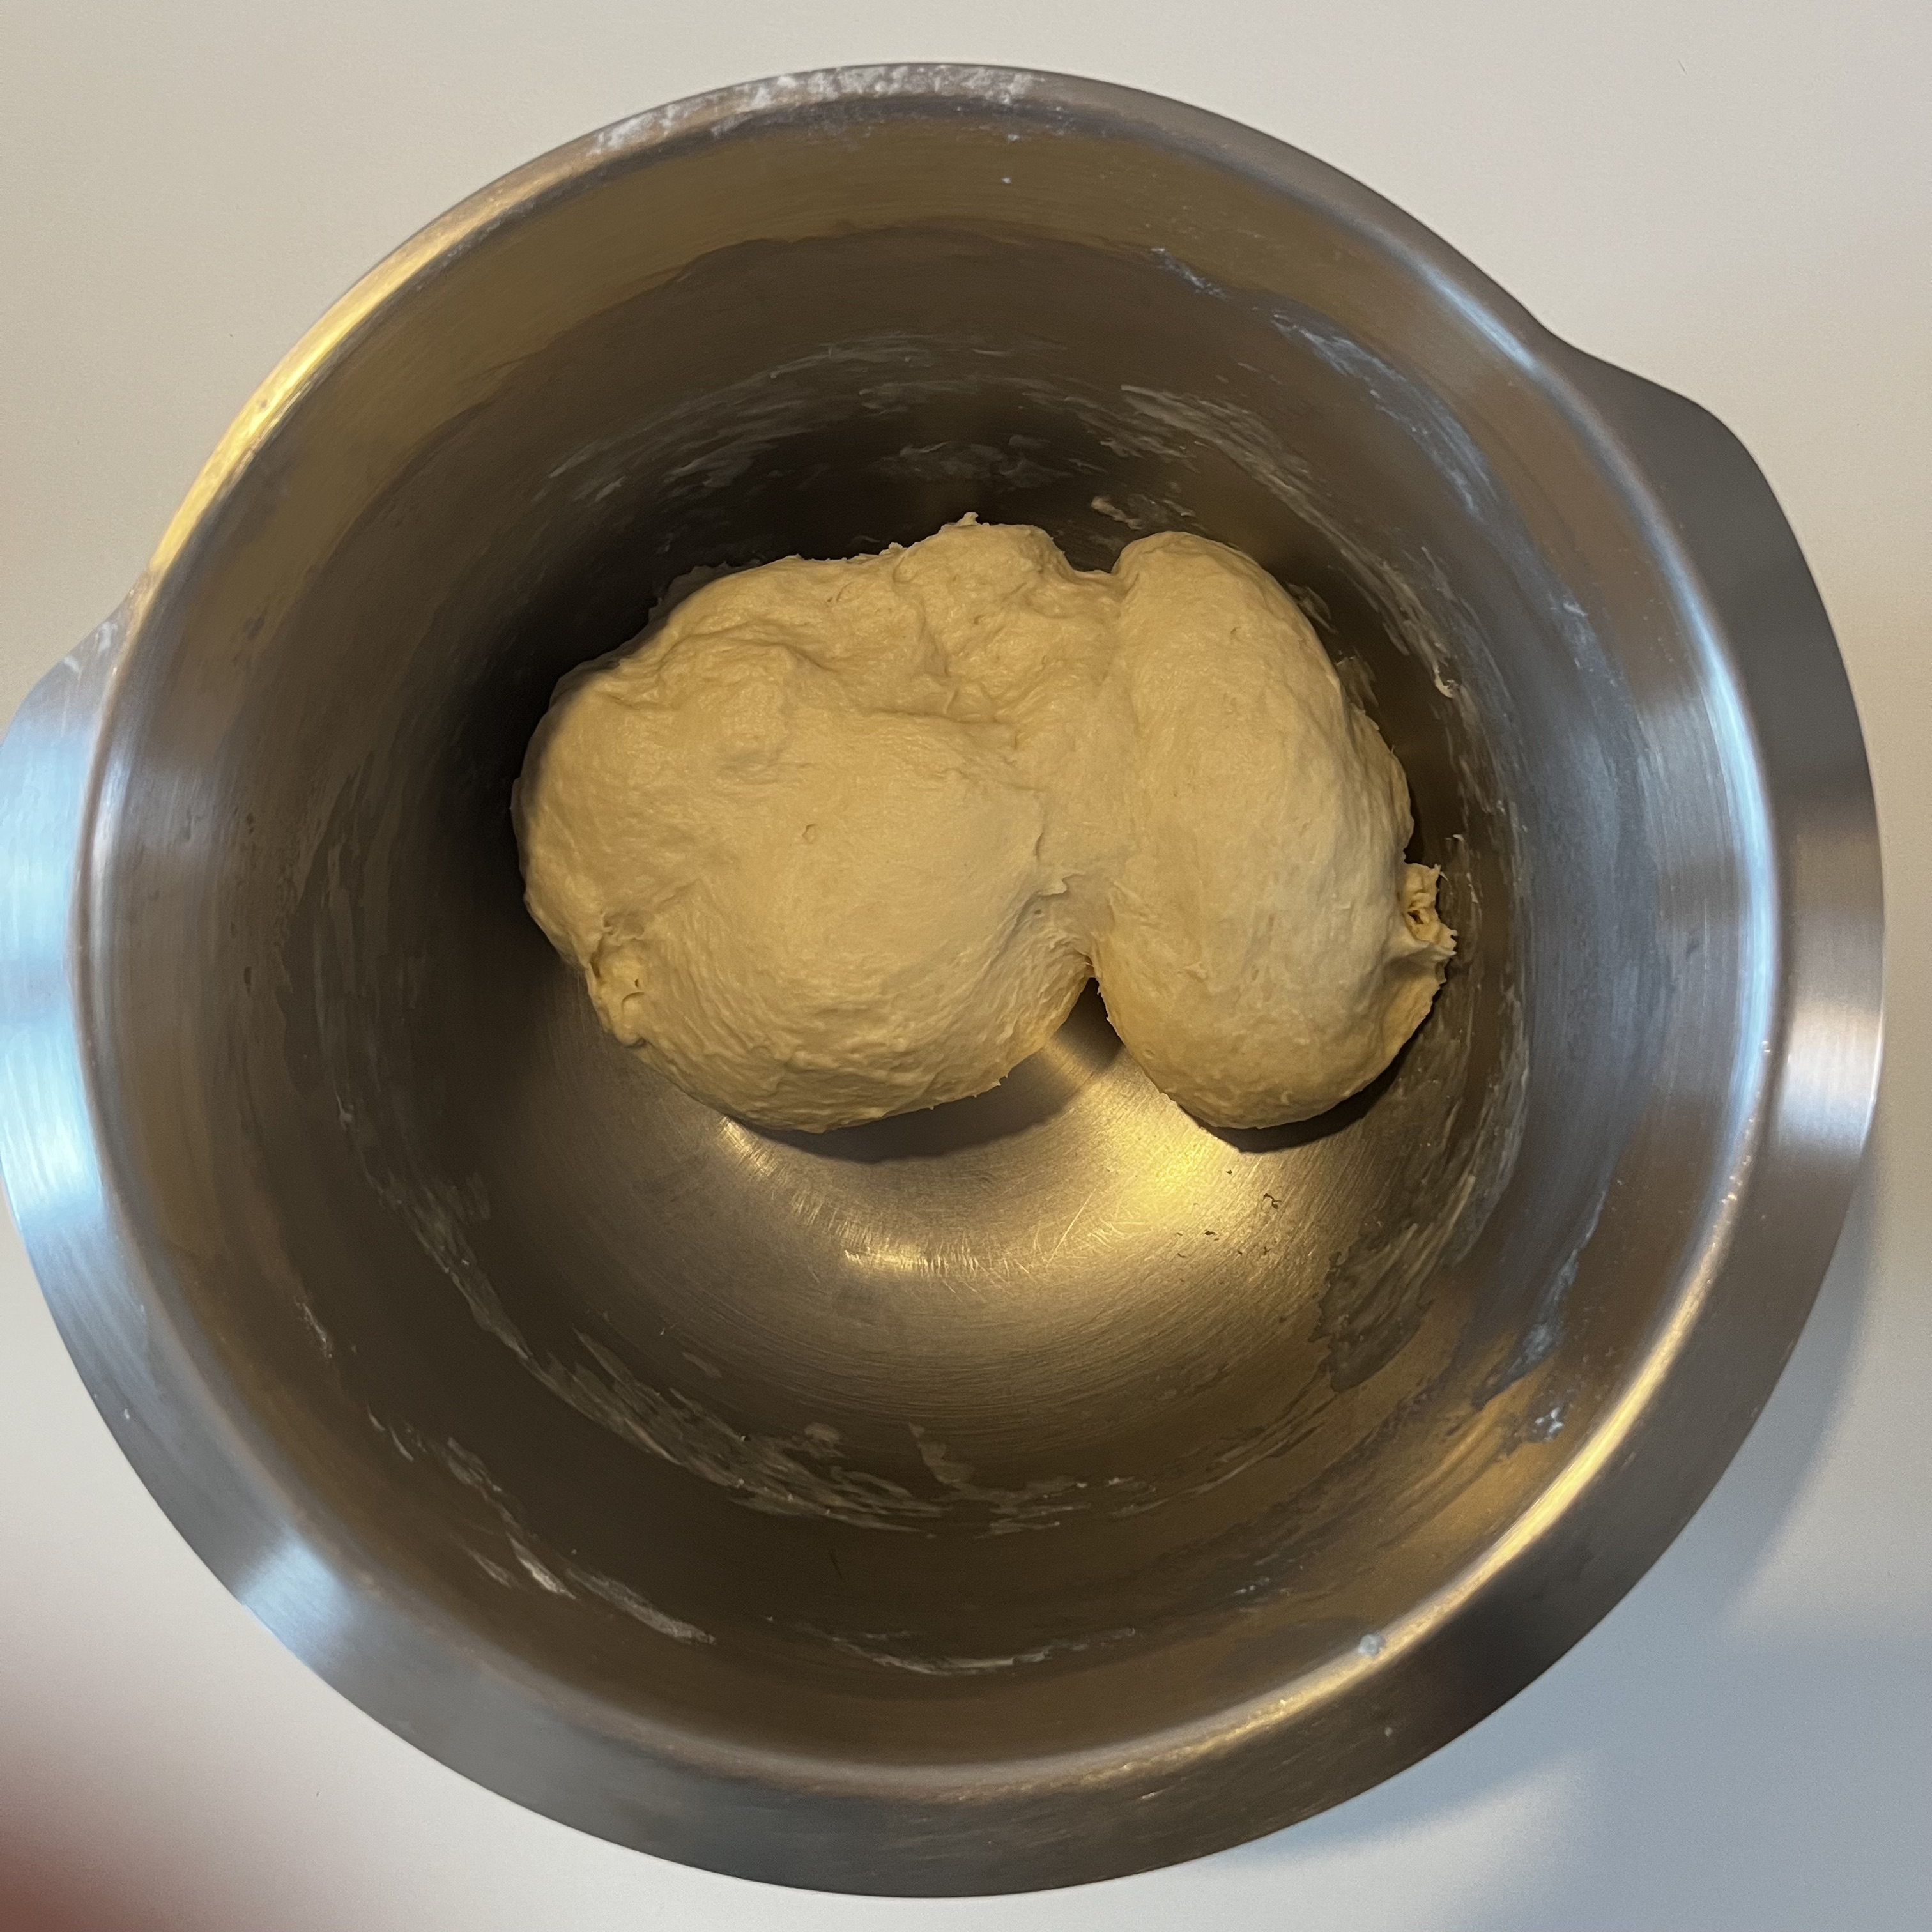
\includegraphics[width=5cm]{figures/IMG_3485}}
  \qquad
  \subfloat[][]{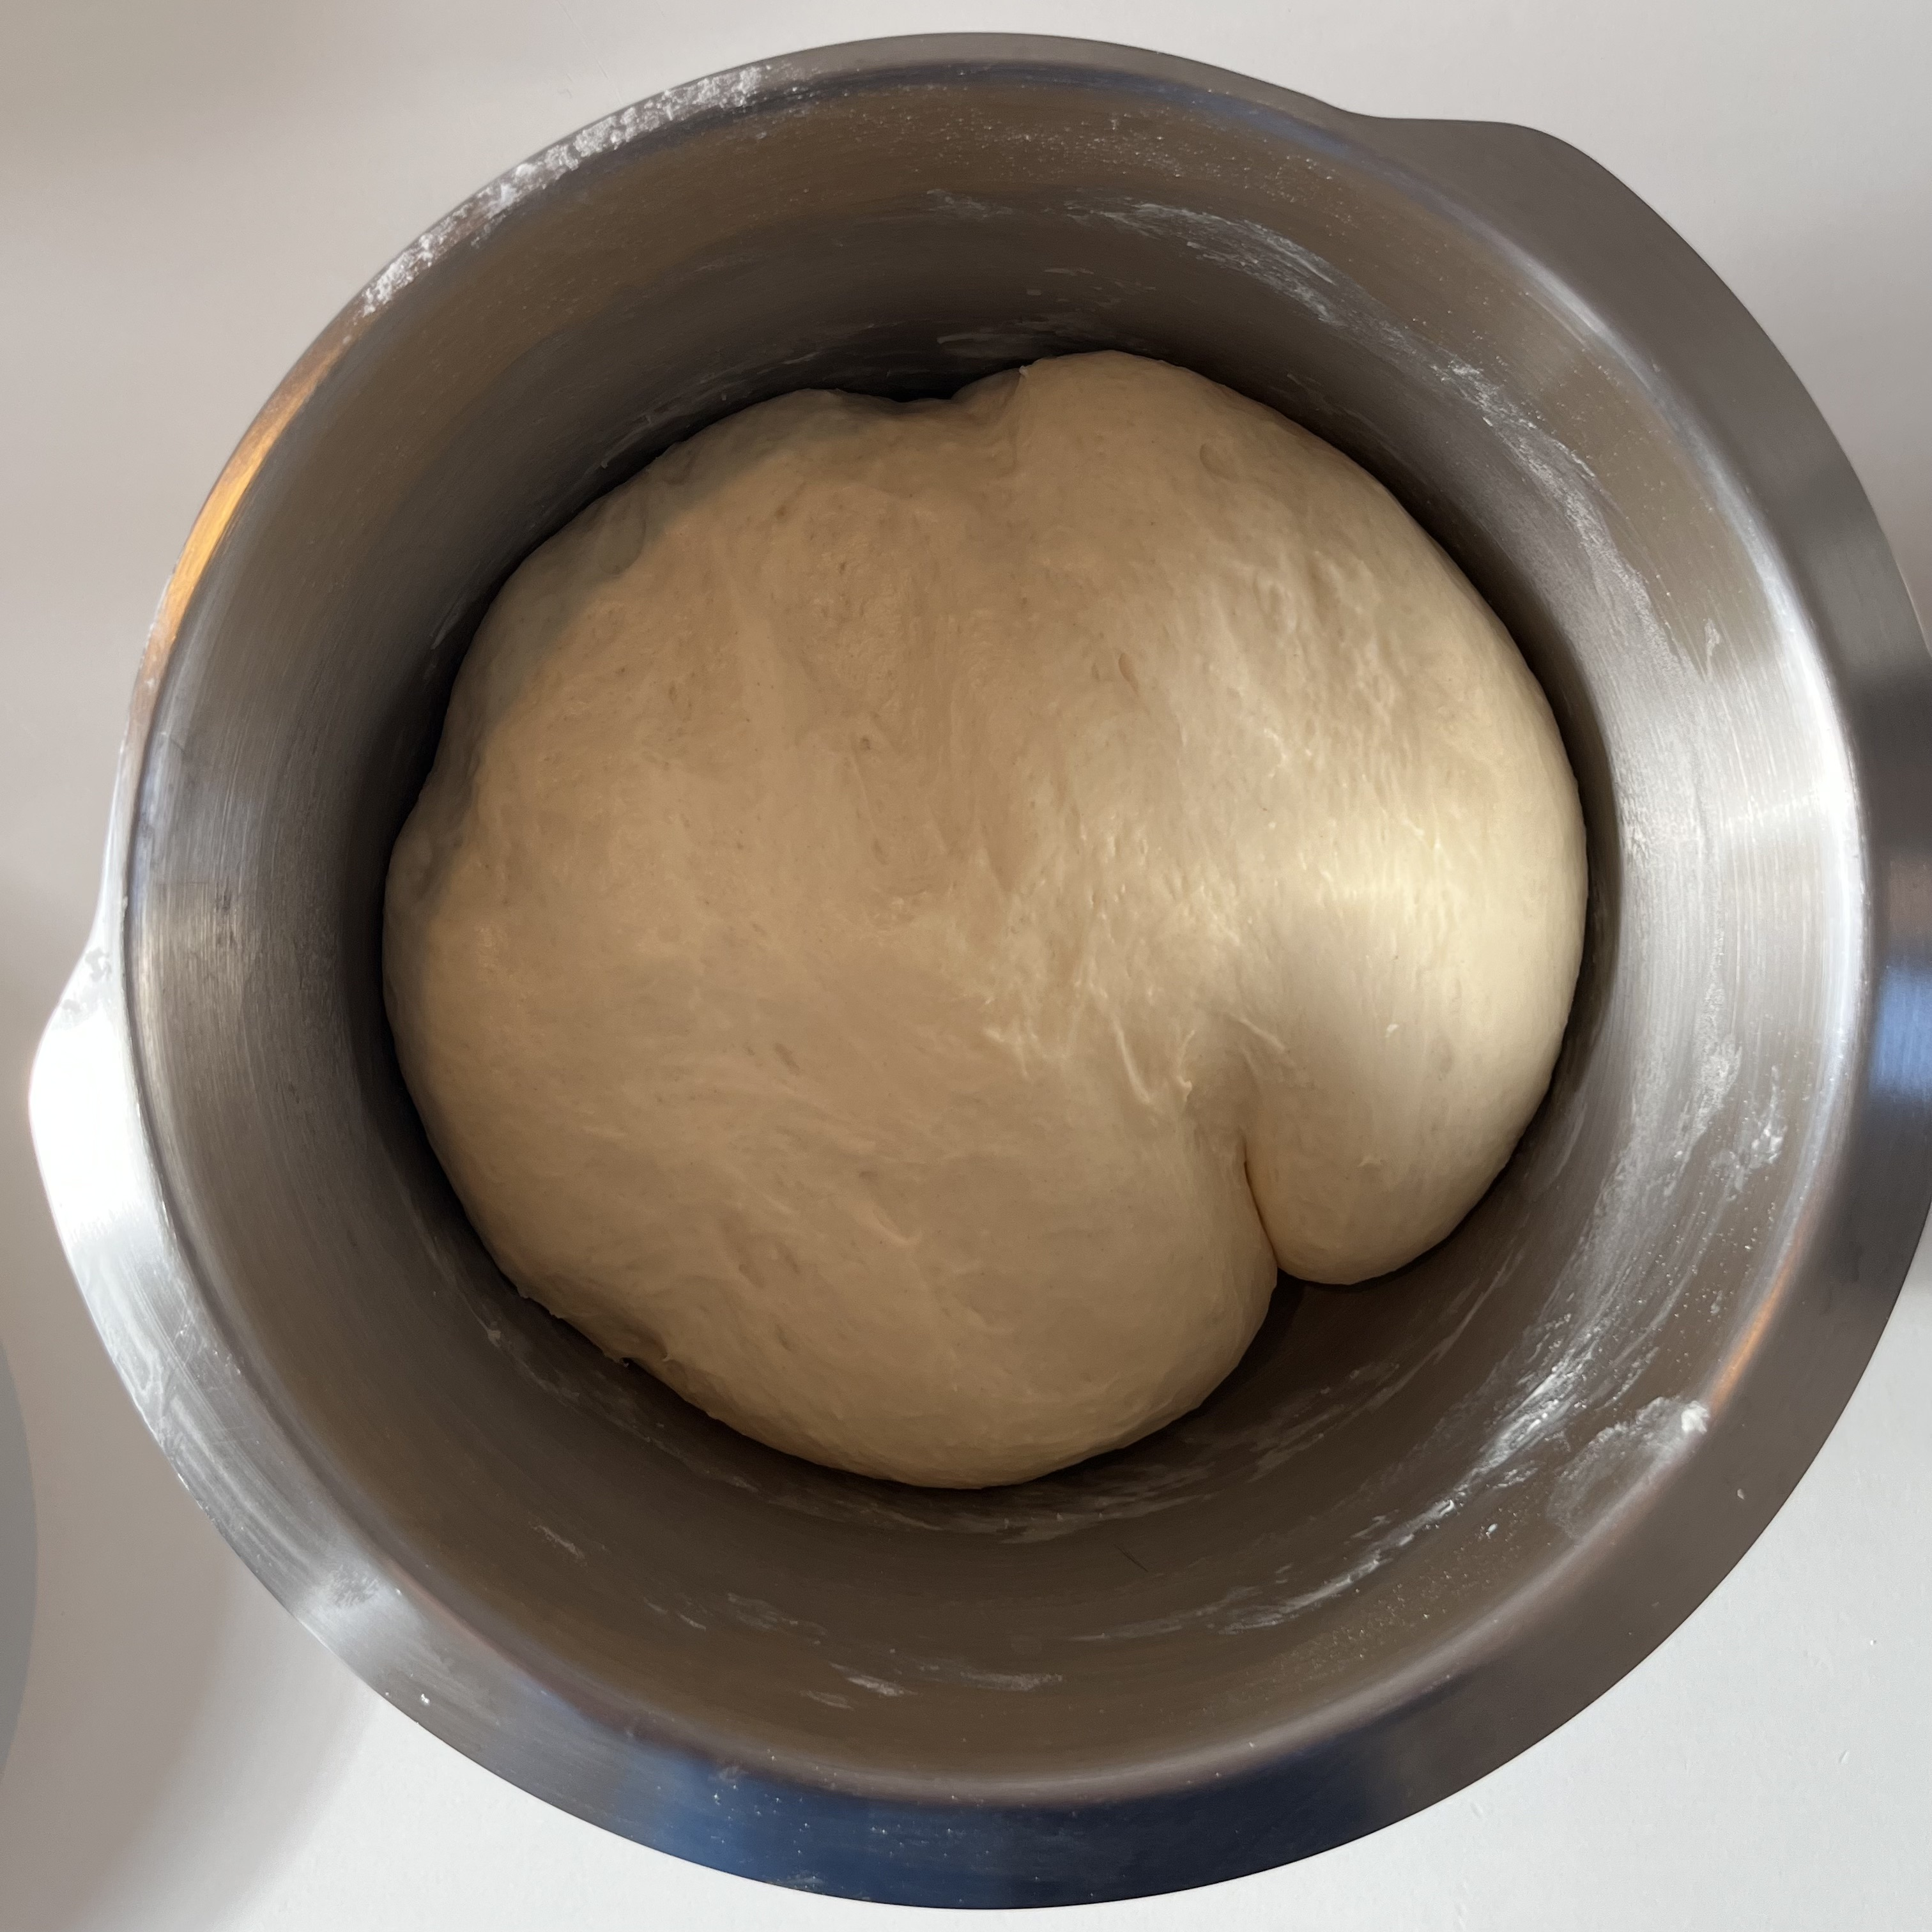
\includegraphics[width=5cm]{figures/IMG_3486}}
  \label{fig:vor_nach_stockgare}
  \caption{Der Teig vor und nach der Stockgare}
\end{figure}

\section*{Füllung}
100 g Butter, 70 g Zucker und 3 TL Zimt in einem Gefäß mit einer Gabel verrühren bis sich eine klebrige Masse gebildet hat. Die Butter muss dabei weich genug sein, um sich verrühren zu lassen, darf aber keinesfalls flüssig sein.

\section*{Zopfherstellung}
\subsection*{Teig ausrollen}
Auf einer leicht bemehlten Arbeitsfläche den Teig von Hand noch 3-4 mal durchkneten und dann zu einem Rechteck mit den Abmessungen 40~cm~$\cdot$~30~cm ausrollen.

\subsection*{Füllung auftragen}
Die gesamte Füllung auf den ausgerollten Teig auftragen. Dabei auf jeder Seite etwa 2~cm Platz lassen. Dieser Rand wird später gebraucht, damit die Rolle zubleibt.

\subsection*{Rollen}
Jetzt vorsichtig über die lange Seite einrollen, sodass sich eine Teigrolle bildet, die eine von der Seite gesehen spiralförmige Füllung enthält. Den Schluss oben etwas andrücken. Je sauberer der Rand ohne Füllung geworden ist, desto besser hält das jetzt.

\subsection*{Flechten}
Das ist der handwerklich schwierigste Teil des Rezepts\footnote{Die Rolle kann auch einfach in Scheiben geschnitten werden, dann hat man Zimtschnecken}, der jedoch kaum Auswirkungen auf den späteren Geschmack hat. \\
Die Teigrolle mit einem scharfen Messer der Länge nach zunächst von einem Ende bis zur Mitte ganz durchschneiden. Dabei sollte der Teig weder plattgedrückt, noch zerrissen werden. Jetzt beiden Zöpfe in sich verdrehen und umeinander schlingen. Den Schluss aufeinander drücken. Im Anschluss die andere Hälfte aufschneiden und auch drehen/flechten. An dieser Stelle empfehle ich das YouTube Video zu Sallys Nusszopf\footnote{\url{https://www.youtube.com/watch?v=YWvEKbcbk2s}} anzuschauen, dort zeigt sie, wie das geht.

\section*{Backen}
\subsection*{Stückgare}
Den Zopf etwa 45 Minuten mit einem Geschirrhandtuch abgedeckt ruhen lassen. In dieser Zeit entspannt sich die Glutenstruktur, sodass er beim Backen nicht reißt. Eventuell geht der Teig noch etwas auf.

\subsection*{Vorheizen}
In der Zwischenzeit den Backofen auf 180 Grad Umluft vorheizen.

\subsection*{Backen}
Den Zopf etwa 20 Minuten backen bis er leicht bräunlich geworden ist.

\section*{Postprocessing}
Etwas abkühlen lassen und mit einer kleisterartigen Mischung aus Puderzucker und wenig Wasser glasieren. Es gibt auch Glasuren aus Frischkäse.

\section*{Lizenz}
\ccbysa{} Creative-Commons-Lizenz\footnote{Um eine Kopie dieser Lizenz zu sehen, besuchen Sie \url{http://creativecommons.org/licenses/by-sa/4.0/}.}.

Dieser Text steht unter der Creative-Commons-Lizenz (\ccLogo) Namensnennung (\ccAttribution) - Weitergabe unter gleichen Bedingungen (\ccShareAlike) 4.0 International. 






\end{document}
